\documentclass{article}

\usepackage{microtype}
\usepackage{graphicx}
\usepackage{subfigure}
\usepackage{booktabs}
\usepackage{amsmath,amsfonts,amssymb}
\usepackage{balance}
\usepackage{hyperref}
\usepackage[accepted]{icml2018}

% For algorithms/pseudocode
\usepackage{algorithm}
\usepackage{algorithmic}

\usepackage{booktabs}   % For \toprule, \midrule, \bottomrule
\usepackage{tabularx}   % For flexible-width columns (X)

% For tikz environment figure
\usepackage{tikz}
\usetikzlibrary{calc,arrows.meta,positioning,decorations.pathreplacing}
\newcommand{\red}[1]{\textcolor{red}{#1}}



% The short title for running headers
\icmltitlerunning{DynaQuant: RL-Based Dynamic Quantization for LLMs}

\begin{document}
	
	\twocolumn[
	\icmltitle{DynaQuant: RL-Based Dynamic Quantization for Large Language Models}
	
	\begin{icmlauthorlist}
		\red{
		\icmlauthor{Oleg Roshka}{stanford}
		\icmlauthor{Ilia Badanin}{epfl}
		shouldn't I be mentioned as an invited collaborator
		}
	\end{icmlauthorlist}
	
	\icmlaffiliation{stanford}{Department of Computer Science, Stanford University, Stanford, CA, USA}
	\icmlaffiliation{epfl}{École Polytechnique Fédérale de Lausanne (EPFL), Lausanne, Switzerland}
	
	\icmlcorrespondingauthor{Oleg Roshka}{oros@stanford.edu}
	\icmlcorrespondingauthor{Ilia Badanin}{ilia.badanin@epfl.ch}
	
	\icmlkeywords{Reinforcement Learning, Quantization, Large Language Models, Memory Efficiency}
	
	\vskip 0.3in
	]
	
	% Print affiliations footnote
	\printAffiliationsAndNotice{}
	
	\begin{abstract}
		Large Language Models (LLMs) often suffer from excessive memory footprints and slow inference, creating barriers to deployment on commodity devices or in high-traffic scenarios. Quantization---using lower numerical precision---is a straightforward way to compress model size, but applying a \emph{uniform} precision (e.g., 8-bit) is suboptimal: some layers tolerate lower precision better than others. We propose \textbf{DynaQuant}, a Reinforcement Learning (RL) framework that \emph{dynamically} selects per-layer quantization schemes (e.g., 4-bit \texttt{nf4}, \texttt{fp4}, \texttt{int8}, or \texttt{fp16}) during short, iterative fine-tuning. Specifically, an RL agent observes each layer's statistics, memory usage, and partial performance signals to choose how to quantize that layer. We employ a multi-term reward that balances perplexity, KL divergence (vs.\ a reference model), attention entropy changes, and memory savings. Experiments on GPT-2 over BoolQ and PIQA show that DynaQuant finds \emph{mixed-precision} assignments that outperform uniform 4-bit or 16-bit baselines in perplexity and accuracy, while still yielding significant memory savings.
	\end{abstract}
	
	\section{Introduction}
	\label{sec:intro}
	Recent progress in Large Language Models (LLMs) has driven state-of-the-art results in various NLP tasks. However, the rapid growth in parameter counts (hundreds of millions to billions of parameters) poses significant memory and runtime challenges, especially for resource-constrained deployments or high-throughput applications. \emph{Quantization} is a practical approach to reduce model size by lowering numerical precision (e.g., from float16 to 8-bit), enabling smaller memory footprints and often faster inference \cite{dettmers2022llmint8,frantar2022gptq}.
	
	Yet, standard uniform quantization assigns the same bit-width to all layers, which can be suboptimal. Some layers—particularly in attention or feed-forward blocks—are more sensitive to precision loss, while others can be safely compressed to 4-bit or even 2-bit with minimal accuracy degradation \cite{dong2019hawq,dettmers2023qlora}. This motivates \emph{mixed-precision quantization}, where each layer's precision is chosen adaptively.
	
	We present \textbf{DynaQuant}, a reinforcement learning (RL) framework that \emph{sequentially} determines each layer's quantization scheme. Specifically:
	\begin{enumerate}
		\item \red{We treat each layer as a step in an RL episode.}
		\item \red{The RL agent selects one action from $\{\texttt{nf4}, \texttt{fp4}, \texttt{int8}, \texttt{fp16}\}$ for that layer.}
		\item \red{After quantizing, we perform a short fine-tuning step on that partially quantized model to mitigate accuracy loss.}
		\item \red{We compute a \emph{reward} that balances perplexity (vs.\ a reference model), KL divergence, attention entropy changes, and memory savings.}
	\end{enumerate}
	By the end of one \emph{episode} (quantizing all layers in sequence), we have a fully quantized model with a \emph{mixed-precision} assignment across layers.
	
	Empirically, we demonstrate that \textbf{DynaQuant} discovers policies that \emph{improve} perplexity and often accuracy relative to uniform 4-bit or 16-bit baselines, with memory usage that falls between those extremes. While our primary experiments use GPT-2 as a testbed, the code also supports other LLMs such as Qwen and Phi-2, and extends readily to additional architectures.
	
	
	\section{Related Work}
	\label{sec:related}
	\paragraph{LLM Quantization.}
	Numerous works compress large models with low-precision formats: int8 \cite{dettmers2022llmint8}, 4-bit normal float (nf4) \cite{frantar2022gptq}, and others \cite{malinovskii2024pvtuning}. Typically, a \emph{uniform} scheme is used. Our approach differs, as we select distinct bit-widths across layers via RL.
	
	\paragraph{Mixed-Precision and NAS.}
	Prior research in Neural Architecture Search (NAS) explores per-layer bit allocations \cite{dong2019hawq,Wang2020apq}, but typically focuses on smaller networks and does not fully account for the \emph{layer-by-layer dynamic impact} of quantization. We adapt these ideas for large Transformer-based LLMs by introducing short, iterative fine-tuning for each layer alongside multi-objective RL signals (e.g., perplexity, KL, memory, attention). Crucially, we fine-tune \emph{both} the quantized model \emph{and} an \emph{episodic reference model} \textbf{after every layer is quantized}, using the same training data for a fixed number of steps. This allows us to precisely capture how quantizing one layer affects subsequent performance—something, to our knowledge, not explored by existing mixed-precision quantization methods for large LLMs.
	
	\paragraph{RL for Model Optimization.}
	Prior works have employed reinforcement learning to discover neural architectures \cite{zoph2016neural} or prune channels \cite{he2018amc}. We build on these techniques by designing a \emph{custom RL environment} tailored to quantizing large Transformer models \emph{layer-by-layer}. In our setup, an agent selects from multiple bit-width formats at each step, and the environment provides a reward based on changes in perplexity, KL divergence, attention entropy, and memory usage. This allows the policy to optimize a \emph{dynamic, multi-term objective} for LLM quantization, rather than applying a static, uniform scheme.
	
	
	\section{Methodology}
	\label{sec:method}
	\subsection{RL Environment: Dynamic Layer Quantization}
	We maintain two models: a reference model $\mathcal{M}_{\text{ref}}$ (e.g., GPT-2 in FP16) and a copy $\mathcal{M}_{\text{quant}}$ for quantization. Each \textbf{episode} processes all $N$ layers in sequence, where each layer corresponds to an RL step:
	
	\begin{enumerate}
		\item \textit{State} $s_i$: incorporates diverse features of the current model and layer. Specifically, we extract:
		\begin{itemize}
			\item \emph{Layer statistics:} mean and standard deviation of weights, gradient norms, and attention entropy for the layer being quantized.
			\item \emph{Global signals:} the normalized layer index $i$, current model perplexity, and perplexity deltas (how quantizing previous layers changed perplexity).
			\item \emph{Previous layer's quantization choice:} encoded as a numeric ratio.
			\item \emph{Exponential moving averages (EWAs):} we maintain running EWAs of key reward components (performance, KL, entropy, memory), smoothing the training signal over steps.
		\end{itemize}
		
		\item \textit{Action} $a_i$: selecting the quantization format from $\{\texttt{nf4}, \texttt{fp4}, \texttt{int8}, \texttt{fp16}\}$ for layer $i$.
		
		\item \textit{Transition}: we quantize layer $i$ in $\mathcal{M}_{\text{quant}}$, then apply \emph{short iterative fine-tuning} on both $\mathcal{M}_{\text{ref}}$ and $\mathcal{M}_{\text{quant}}$, using the \emph{identical} mini-batch for a fixed number of steps. This ensures the agent observes the immediate impact of quantizing that layer.
		
		\item \textit{Reward} $r_i$: once both models are briefly fine-tuned, we measure the resulting perplexities, KL divergence, attention entropy, and memory savings. These are combined (with EWAs) into a multi-term scalar reward. While memory usage is not directly encoded in the state representation, the \emph{reward} incorporates memory efficiency by considering the bits saved through quantization, scaled by the relative size of the current layer.
	\end{enumerate}
	
	At the end of all $N$ layers, the environment signals the episode is complete and the PPO agent updates its policy using the collected trajectory. This cycle repeats until the agent converges on an effective per-layer quantization policy.
	
	\begin{figure}[t]
		\centering
		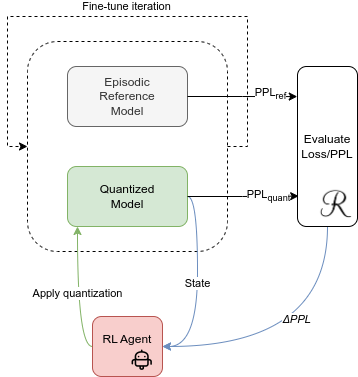
\includegraphics[width=0.95\linewidth]{images/dynaq-scheme.png}
		\vspace{-0.5em}
		\caption{\small RL-based dynamic quantization loop. The agent selects a quantization type for the current layer, we fine-tune the quantized and reference models, then compute performance signals and memory usage to form a reward.}
		\label{fig:rl-env}
		\vspace{-0.5em}
	\end{figure}

    \subsection{Reward Design}
    \label{subsec:reward}
    
    Our reward function for layer \(i\), denoted \(r_i\), is a weighted sum of four terms capturing performance, divergence, attention preservation, and memory savings:
    
    \paragraph{(1) Performance (Perplexity) Reward.}
    We compare the perplexities of the reference model (\(\mathrm{PPL}_\text{ref}\)) and the quantized model (\(\mathrm{PPL}_\text{quant}\)):
    \begin{equation}
    	r_{\mathrm{perf}} 
    	\,=\, 
    	\Bigl(\mathrm{PPL}_\text{ref} - \mathrm{PPL}_\text{quant}\Bigr)
    	\,\times\, 
    	w_{\mathrm{perf}}.
    	\label{eq:perf_term}
    \end{equation}
    If quantization reduces perplexity below that of the reference, \(r_{\mathrm{perf}}\) is positive; otherwise, it is typically negative.
    
    \paragraph{(2) KL Divergence Penalty.}
    To penalize large deviations in predictive distributions, we compute:
    \begin{equation}
    	r_{\mathrm{KL}} 
    	\,=\, 
    	-\, w_{\mathrm{KL}} 
    	\,\times\, 
    	\mathrm{KL}\bigl(p_\text{quant}\,\|\,p_\text{ref}\bigr),
    \end{equation}
    where \(p_\text{quant}\) and \(p_\text{ref}\) are the output distributions (softmax of the logits) from the quantized and reference models, respectively. A higher KL divergence incurs a larger negative reward.
    
    \paragraph{(3) Attention Entropy Preservation.}
    Retaining rich attention patterns can be crucial for model quality. We quantify this by comparing the attention entropies of layer \(i\) in both models:
    \begin{equation}
    	r_{\mathrm{entropy}} 
    	\,=\, 
    	\bigl(E_\text{quant} - E_\text{ref}\bigr)
    	\,\times\, 
    	w_{\mathrm{entropy}},
    \end{equation}
    where \(E_\text{quant}\) and \(E_\text{ref}\) denote the mean attention entropy in the current layer for the quantized and reference models, respectively.
    
    \paragraph{(4) Memory Savings.}
    Finally, we reward bit savings relative to a 16-bit baseline. For each parameter in layer \(i\), the agent saves \(16 - \text{bits}(a_i)\) bits if action \(a_i\) is chosen. This is weighted by the fraction of total parameters in layer \(i\), denoted \(\text{layer\_size\_ratio}_i\):
    \begin{equation}
    	r_{\mathrm{mem}} 
    	\,=\, 
    	\Bigl(\frac{16 - \text{bits}(a_i)}{16}\Bigr)
    	\,\times\,
    	\text{layer\_size\_ratio}_i
    	\,\times\, 
    	w_{\mathrm{memory}}.
    \end{equation}
    Here we define
    \[
    \text{layer\_size\_ratio}_i 
    \,=\, 
    \frac{\text{numParams}(i)}{\text{numParams}(\text{model})},
    \]
    so that layers with more parameters yield proportionally higher savings.
        
    The final reward for layer \(i\) combines all terms:
    \begin{equation}
    	\label{eq:reward_final}
    	r_i 
    	\,=\,
    	r_{\mathrm{perf}} 
    	\,+\, 
    	r_{\mathrm{KL}} 
    	\,+\, 
    	r_{\mathrm{entropy}} 
    	\,+\, 
    	r_{\mathrm{mem}}.
    \end{equation}
    By adjusting the weights \(w_{\mathrm{perf}}, w_{\mathrm{KL}}, w_{\mathrm{entropy}},\) and \(w_{\mathrm{memory}}\), practitioners can prioritize different trade-offs between model fidelity and compression.
    		
	\subsection{Policy Learning via PPO}
	We employ \textbf{Proximal Policy Optimization (PPO)} \cite{ppo2017} to update a small MLP policy $\pi_\theta$ that maps states to discrete actions (quantization types). At each new \emph{episode}, we:
	\begin{enumerate}
		\item \emph{Reset} the environment: copy the reference model to reinitialize $\mathcal{M}_\text{quant}$, set layer index to 0.
		\item For each layer $i=0 \dots N-1$:
		\begin{itemize}
			\item Agent picks $a_i \sim \pi_\theta(\cdot|s_i)$.
			\item We apply quantization type $a_i$ to layer $i$, perform short fine-tuning, measure $(\mathrm{PPL}_\text{quant}, \mathrm{PPL}_\text{ref}, \mathrm{KL}, E_\text{quant}, E_\text{ref})$, compute reward $r_i$.
			\item Next state $s_{i+1}$ updated with new stats, layer index, etc.
		\end{itemize}
		\item We collect $(s_i,a_i,r_i)$ for all $i$, compute advantages (e.g., GAE), and run a few epochs of PPO updates on $\pi_\theta$.
	\end{enumerate}
	
	\vspace{-0.75em}
	\subsection{Algorithmic Pseudocode}
	\label{subsec:pseudocode}
	\vspace{-0.25em}
	
	\begin{algorithm}[h]
		\footnotesize
		\caption{DynaQuant (One PPO Iteration)}
		\label{alg:dynaquant}
		\begin{algorithmic}[1]
			\REQUIRE Model $\mathcal{M}_\text{ref}$ (baseline), RL policy $\pi_\theta$, reward weights $(w_{\mathrm{perf}}, w_{\mathrm{KL}}, w_{\mathrm{entropy}}, w_{\mathrm{memory}})$
			\STATE $\mathcal{M}_\text{quant} \leftarrow \text{clone of } \mathcal{M}_\text{ref}$
			\STATE $s_0 \leftarrow \textsc{InitState}()$; $i \leftarrow 0$; \text{done} $\leftarrow$ \textbf{False}
			\STATE \texttt{rollout} $\leftarrow []$
			\WHILE{not \text{done}}
			\STATE $a_i \sim \pi_\theta(a_i|s_i)$
			\STATE \textsc{QuantizeLayer}$(\mathcal{M}_\text{quant}, i, a_i)$
			\STATE \textsc{FineTune}($\mathcal{M}_\text{ref}, \text{dataBatch}, \text{epochs})$
			\STATE \textsc{FineTune}($\mathcal{M}_\text{quant}, \text{dataBatch}, \text{epochs})$
			\STATE $(r_i, \text{info}_i) \leftarrow \textsc{ComputeReward}(\mathcal{M}_\text{ref}, \mathcal{M}_\text{quant}, i)$
			\STATE $s_{i+1} \leftarrow \textsc{NextState}(\mathcal{M}_\text{quant}, i+1)$
			\STATE \texttt{rollout} $\leftarrow \texttt{rollout}\cup \{(s_i,a_i,r_i)\}$
			\STATE $i \leftarrow i+1$
			\IF{$i \ge N$}
			\STATE done $\leftarrow$ \textbf{True}
			\ENDIF
			\ENDWHILE
			\STATE \textsc{ComputeAdvantages}(\texttt{rollout})
			\STATE \textsc{UpdatePolicyPPO}($\pi_\theta$, \texttt{rollout})
		\end{algorithmic}
	\end{algorithm}
	
	Algorithm~\ref{alg:dynaquant} shows a single training iteration (episode). We typically repeat many episodes, reinitializing $\mathcal{M}_\text{quant}$ and $\mathcal{M}_\text{ref}$ each time.
	
	\section{Experiments}
	\label{sec:experiments}
	
	\subsection{Setup and Datasets}
	
	\paragraph{Reference Model.}
	We begin with GPT-2 (12-layer) as our base model, fine-tuning it on CommonsenseQA using standard procedures (e.g., AdamW optimizer for several epochs) to produce an FP16 \emph{reference model}. This serves as the foundation for all subsequent quantization.
	
	\paragraph{Quantization Approach.}
	All experiments---including both baselines and our RL-driven policy---use the same in-house quantization utilities. These support 4-bit (nf4/fp4) and 8-bit (int8) formats, as well as FP16/FP32 copy operations. This ensures consistent layer-wise transforms for both training and evaluation, so that any performance difference stems purely from how bits are allocated per layer, rather than from mismatched quantization methods.
	
	\paragraph{Tasks.}
	We evaluate on two downstream benchmarks:
	\begin{itemize}
		\item \textbf{BoolQ}: binary (yes/no) reading comprehension,
		\item \textbf{PIQA}: a multiple-choice physical reasoning dataset.
	\end{itemize}
	\red{remove this part below}
	Both are assessed on publicly available validation sets, where we measure:
	\begin{enumerate}
		\item \emph{Validation perplexity}, computed as the exponentiated mean cross-entropy over either the full or chunked sequences,
		\item \emph{Multiple-choice accuracy}, where each choice is scored via negative cross-entropy and the highest-likelihood answer is selected,
		\item \emph{Peak GPU memory usage} (MB), obtained by monitoring allocated memory before and after a forward pass,
		\item \emph{Inference throughput} (tokens/s), measured by timing multiple forward passes over synthetic token batches.
	\end{enumerate}
	
	\subsection{Baselines and Evaluation Methodology}
	
	\paragraph{Uniform Precision Baselines.}
	\textbf{Uniform FP16} directly uses the fine-tuned reference model. For \textbf{Uniform NF4}, the same reference model is converted to 4-bit across every linear layer in one uniform pass. In both cases, the underlying weights, hyperparameters, and training data remain identical, differing only in their final precision.
	
	\paragraph{RL-Based Mixed Precision.}
	Our proposed \textbf{DynaQuant} uses a reinforcement learning policy to assign different bit-widths on a per-layer basis. After policy training, the layer-wise quantization scheme is finalized and applied to the reference model. The rest of the architecture and training data remain unchanged, ensuring a fair comparison with uniform baselines.
	
	\paragraph{Evaluation Procedure.}
	We evaluate all models---FP16, NF4, and RL-based mixed precision---through the same pipeline. We load the final model checkpoint (either reference or quantized) into GPT-2 and apply our quantization utilities as needed. For evaluation, we calculate validation perplexity on the dataset using token-level cross-entropy. To assess multiple-choice accuracy, we score each candidate answer and select the one with the lowest average cross-entropy. Finally, we measure inference performance by recording throughput and peak memory usage across repeated forward passes using synthetic input batches.
	
	By standardizing the quantization routines, data preprocessing, and evaluation scripts across all settings, we ensure that any observed differences in performance or memory usage reflect genuine trade-offs arising from the chosen precision formats.
	
	\subsection{Loss Metrics}
	\begin{figure}[ht]
		\centering
		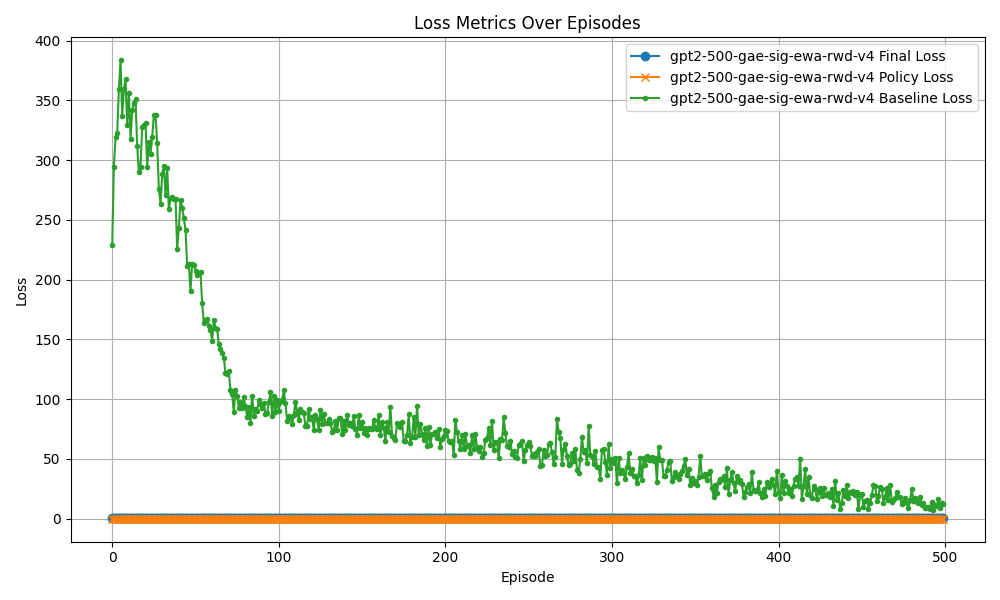
\includegraphics[width=\columnwidth]{gpt2-500-gae-sig-ewa-rwd-v4-losses.png}
		\vspace{-1em}
		\caption{\small
			\red{use a better graph. mention a model, \#epochs, dataset}
			Three separate loss values over 500 training episodes:
			\textbf{(blue)} the final validation loss (``final\_loss'') of the quantized model after each episode,
			\textbf{(orange)} the policy loss (the PPO objective),
			\textbf{(green)} the baseline loss (the value function’s MSE).}
		\label{fig:loss_curves}
		\vspace{-0.2em}
	\end{figure}
	
	Figure~\ref{fig:loss_curves} tracks three distinct metrics logged each episode:
	\red{this explanation is stupid; should be replaced.}
	\begin{itemize}
		\item \textbf{Final Validation Loss (Blue).} 
		After each full episode (i.e., once all layers have been quantized), we compute the quantized model's validation loss (cross-entropy). 
		In our runs, this loss remains close to zero or very small on the chosen scale, indicating the model’s performance does not degrade severely despite aggressive mixed-precision.
		
		\item \textbf{Policy Loss (Orange).} 
		This is the PPO objective we optimize when updating the quantization policy. 
		It typically fluctuates early on as the agent explores different quantization schemes, then settles near zero, suggesting the policy has converged to stable decisions.
		
		\item \textbf{Baseline Loss (Green).}		
		This is the MSE of the “baseline network” used in PPO to estimate state values. 
		We see it starts high, briefly spikes, and then gradually decreases, reflecting the baseline’s learning to predict returns more accurately over time.
	\end{itemize}
	
	In summary, the orange policy loss and blue final loss both end near zero, while the green baseline loss steadily declines from large initial values. 
	This pattern indicates that \emph{(1)} the quantization policy stabilizes, \emph{(2)} the value-function baseline converges, and \emph{(3)} the final quantized model maintains strong performance (low validation loss). 
		
	\subsection{Total Reward Curve}
	\begin{figure}[ht]
	\centering
	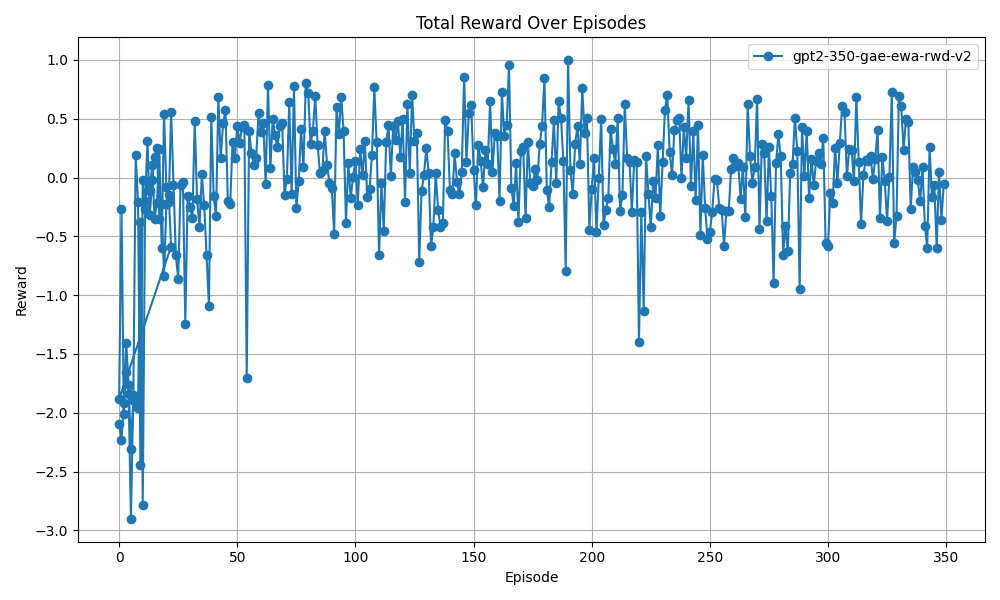
\includegraphics[width=\columnwidth]{gpt2-350-gae-ewa-rwd-v2-reward.png}
	\vspace{-1em}
	\caption{\small Example of total reward vs.\ episode. The agent steadily improves as it refines its per-layer quantization decisions.}
	\label{fig:reward_curves}
	\vspace{-0.2em}
	\end{figure}	
	
	\red{this explanation is stupid; should be merged with the previous part.}
	
	Figure~\ref{fig:reward_curves} illustrates how the \emph{total reward} evolves with each training episode. Recall that our reward encompasses perplexity differences (versus the reference model), KL divergence, attention entropy, and memory savings. 
	
	\begin{itemize}
		\item \textbf{Initial Negative Values.} Early episodes yield negative rewards, as random or naive quantization decisions often deteriorate performance substantially.
		\item \textbf{Steady Improvement.} Within a few dozen episodes, the agent discovers beneficial bit assignments that yield moderate memory savings with minimal perplexity increase, driving the reward into positive territory.
		\item \textbf{Late Stabilization.} Beyond 150--200 episodes, most runs hover around slightly above zero reward, reflecting a stable trade-off between memory gains and model fidelity.
	\end{itemize}
	
	This steady rise confirms that the RL agent effectively learns how to balance precision requirements with compression targets.
	
	\subsection{Layer-Wise Quantization Distribution}
	
	\begin{figure}[ht]
		\centering
		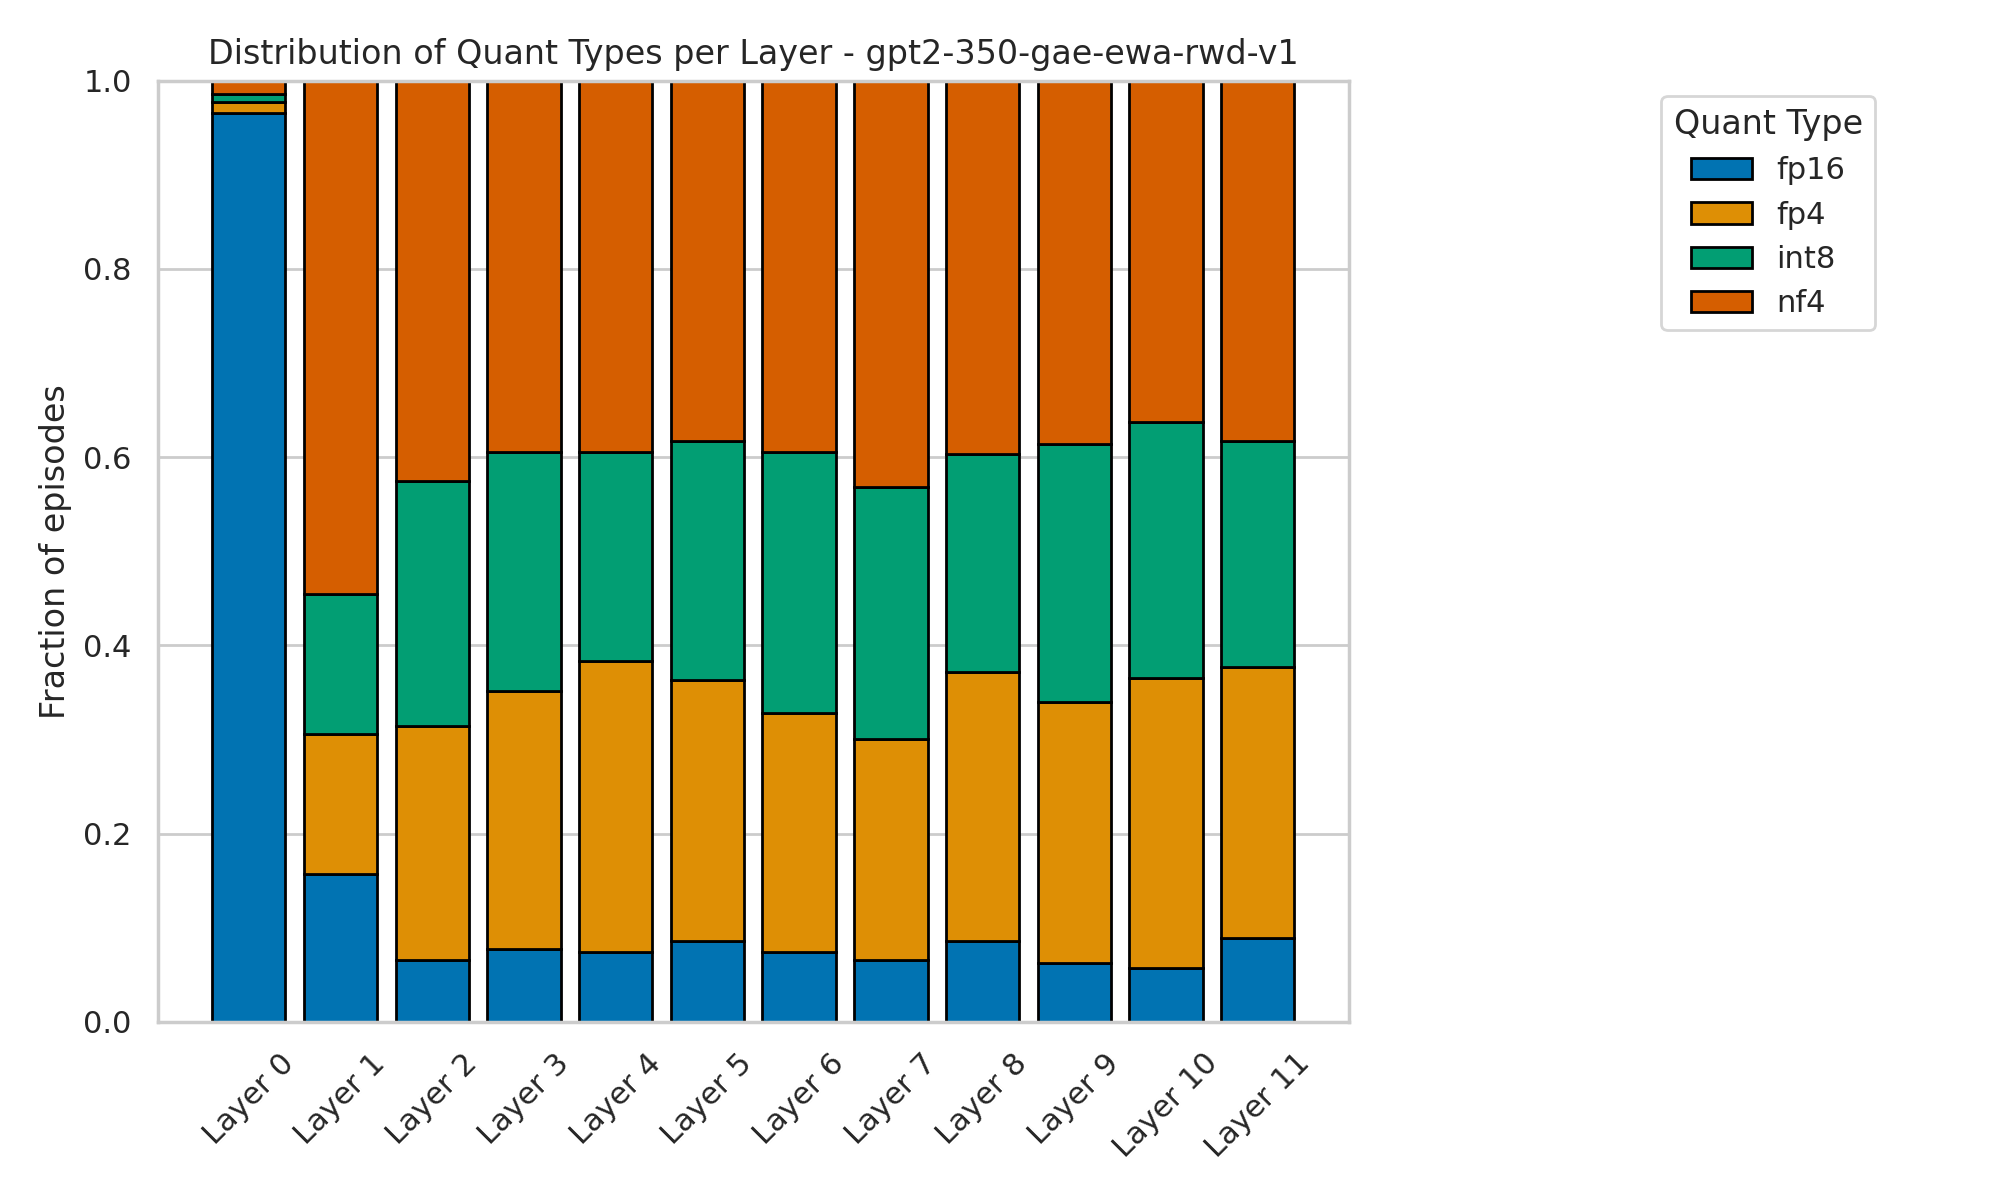
\includegraphics[width=0.93\columnwidth]{gpt2-350-gae-ewa-rwd-v1_quant_dist_bar.png}
		\vspace{-0.4em}
		\caption{\small Quantization type distribution across layers \red{shouldd include more information}}
		\label{fig:bardist}
		\vspace{-0.5em}
	\end{figure}
	
	\begin{figure}[ht]
		\centering
		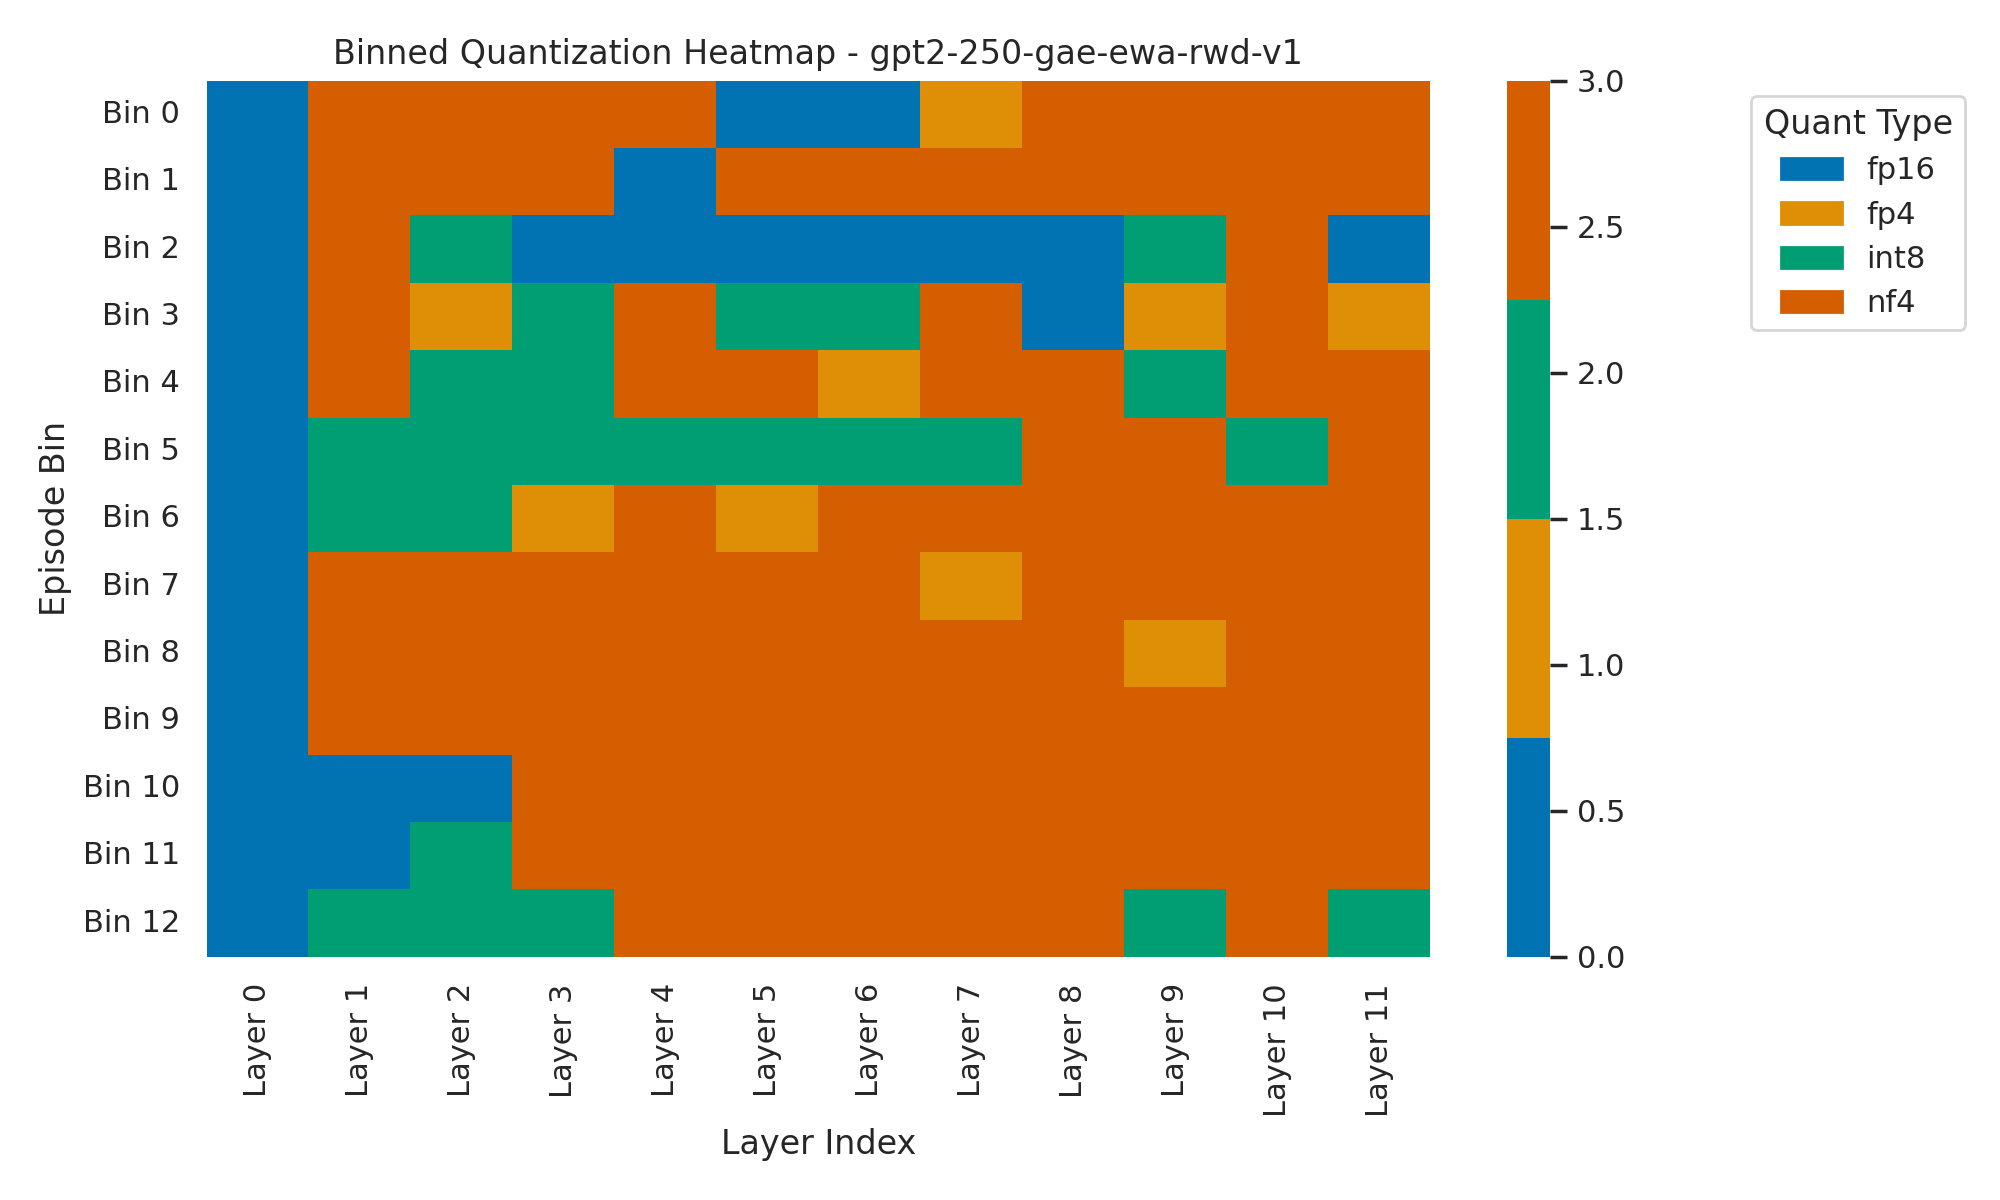
\includegraphics[width=0.93\columnwidth]{gpt2-250-gae-ewa-rwd-v1_quant_heatmap_binned.png}
		\vspace{-0.4em}
		\caption{\small Heatmap showing quantization type usage by layer across binned episodes. The RL policy typically picks lower bits for many layers, using higher precision on sensitive blocks.}
		\label{fig:bin_heatmap}
		\vspace{-0.5em}
	\end{figure}
	
	We next examine how often each layer is assigned a particular bit-width once the policy converges. Figures~\ref{fig:bardist} and~\ref{fig:bin_heatmap} visualize the final distribution of quantization formats across 12 Transformer layers:
	
	\begin{itemize}
		\item \textbf{Distribution Bar Chart (Figure~\ref{fig:bardist}).} Each column corresponds to a layer, and each color segment in the column shows the fraction of episodes for which that layer was assigned \texttt{fp16}, \texttt{fp4}, \texttt{int8}, or \texttt{nf4}. We observe that some layers predominantly end up in 4-bit or 8-bit formats, while others remain in \texttt{fp16}. This layer-specific pattern suggests certain layers are more sensitive to precision reduction.
		\item \textbf{Binned Heatmap (Figure~\ref{fig:bin_heatmap}).} Episodes are grouped into bins on the vertical axis, and layers are shown horizontally. The color indicates the chosen quantization type. Early in training, many layers fluctuate. As training progresses (moving down the vertical axis), the agent "locks in" stable choices, with orange (\texttt{nf4}) and green (\texttt{int8}) dominating most layers, while a few sensitive blocks remain in \texttt{fp16}.
	\end{itemize}
	
	Both plots confirm that the RL policy \emph{does not} rely on a uniformly lower bit-width. Instead, it actively tailors the format per layer, highlighting the benefit of dynamic quantization.
	
	\paragraph{Interpretation.}
	Altogether, these results indicate that different transformer layers \emph{vary} in their robustness to low-bit quantization. The agent learns to compress most layers (often with 4-bit or 8-bit) while retaining higher precision where needed. As a result, overall memory usage is significantly reduced, with only a marginal hit to validation loss compared to a purely FP16 baseline.
			
	
	\section{Results}
	
	\red{can you elaborate on what the mix A, B, C, D are?}
	
	\subsection{Results on BoolQ (GPT-2 Small)}
	
	\begin{table}[ht]
		\centering		
		\label{tab:boolq-small}
		\begin{tabular}{lcccc}
			\toprule
			\textbf{Method} & \textbf{PPL}$\downarrow$ & \textbf{Acc(\%)}$\uparrow$ & \textbf{Mem(MB)}$\downarrow$ \\
			\midrule
			\textbf{FP16 (baseline)}  & 920.56 & 51.93 & 422.69 \\
			\textbf{NF4 (uniform)}    & 873.65 & 52.02 & \textbf{300.95} \\
			\midrule
			\textbf{DynaQ Mix A}      & 777.13 & 52.08 & 464.29 \\
			\textbf{DynaQ Mix B}      & \textbf{773.78} & \textbf{53.85} & 383.15 \\
			\bottomrule
		\end{tabular}
		\caption{\small BoolQ validation results for GPT-2 Small. The first two rows show uniform quantization baselines (FP16 and NF4). The remaining rows demonstrate our learned DynaQuant mixed-precision schemes that adaptively quantize different layers.}
	\end{table}
	
	\paragraph{Observations for GPT-2 Small on BoolQ.}
	From Table~\ref{tab:boolq-small}, uniform NF4 beats FP16 in perplexity (873.65 vs.\ 920.56) with notably lower memory usage (300.95~MB vs.\ 422.69~MB). Our RL approach (e.g., DynaQ Mix B) lowers perplexity further \emph{and} boosts accuracy significantly (53.85\% vs.\ NF4’s 52.02\%), though at a slight memory overhead (383.15~MB vs.\ NF4’s 300.95~MB).
	
	%----------------------------------------------
	\subsection{Results on PIQA (GPT-2 Small)}
	
	\begin{table}[ht]
		\centering
		\label{tab:piqa-small}
		\begin{tabular}{lcccc}
			\toprule
			\textbf{Method} & \textbf{PPL}$\downarrow$ & \textbf{Acc(\%)}$\uparrow$ & \textbf{Mem(MB)}$\downarrow$ \\
			\midrule
			\textbf{FP16}    & 2531.21 & 60.72 & 422.69 \\
			\textbf{NF4}     & 2265.88 & 60.77 & \textbf{300.95} \\
			\midrule
			\textbf{DynaQ Mix C} & 2143.76 & \textbf{61.53} & 464.29 \\
			\textbf{DynaQ Mix D} & \textbf{2099.65} & 61.26 & 383.15 \\
			\bottomrule
		\end{tabular}
		\caption{\small PIQA validation results for GPT-2 Small. The first two rows show uniform quantization baselines (FP16 and NF4). The remaining rows demonstrate our learned DynaQuant mixed-precision schemes.}
	\end{table}
	
	\paragraph{Observations for GPT-2 Small on PIQA.}
	Table~\ref{tab:piqa-small} shows a similar trend. Uniform NF4 again outperforms FP16 in perplexity (2265.88 vs.\ 2531.21) with lower memory usage. \emph{Mix C} yields the highest accuracy (61.53\%) but also the highest memory usage among these methods (464.29~MB). \emph{Mix D} maintains a perplexity of 2099.65 and slightly lower accuracy, at a memory cost well below FP16.
	
	%----------------------------------------------
	\subsection{Results on BoolQ (GPT-2 Medium)}
	
	\begin{table}[ht]
		\centering
		\label{tab:boolq-medium}
		\begin{tabular}{lcccc}
			\toprule
			\textbf{Method} & \textbf{PPL}$\downarrow$ & \textbf{Acc(\%)}$\uparrow$ & \textbf{Mem(MB)}$\downarrow$ \\
			\midrule
			\textbf{FP16 (baseline)}  & 1009.31 & 54.22 & 956.26 \\
			\textbf{NF4 (uniform)}    & \textbf{953.16}  & 54.53 & 513.04 \\
			\midrule
			\textbf{DynaQ Mix A}      & 1094.60 & \textbf{54.80} & 694.23 \\
			\textbf{DynaQ Mix B}      & 1091.37 & 54.71 & 622.10 \\
			\textbf{DynaQ Mix C}      & 978.64  & 54.71 & \textbf{532.71} \\
			\bottomrule
		\end{tabular}
		\caption{\small BoolQ validation results for GPT-2 Medium. The first two rows show uniform quantization baselines (FP16 and NF4). The remaining rows demonstrate our learned DynaQuant mixed-precision schemes.}
	\end{table}
	
	\paragraph{Observations for GPT-2 Medium on BoolQ.}
	As in the smaller model, uniform NF4 beats FP16 in perplexity (953.16 vs.\ 1009.31) at about half the memory footprint (513~MB vs.\ 956~MB). Several mixes (e.g., Mix A) slightly boost accuracy to 54.80\% but can raise memory usage. Notably, Mix C dips below the uniform NF4 perplexity (978.64 vs.\ 953.16) but remains comparable in accuracy.
	
	%----------------------------------------------
	\subsection{Results on PIQA (GPT-2 Medium)}
		
	\begin{table}[ht]
		\centering
		\label{tab:piqa-medium}
		\begin{tabular}{lcccc}
			\toprule
			\textbf{Method} & \textbf{PPL}$\downarrow$ & \textbf{Acc(\%)}$\uparrow$ & \textbf{Mem(MB)}$\downarrow$ \\
			\midrule
			\textbf{FP16 (baseline)} & 5791.41 & \textbf{64.58} & 956.26 \\
			\textbf{NF4 (uniform)}   & 4932.96 & 64.53 & 513.04 \\
			\midrule
			\textbf{DynaQ Mix A}     & 5399.04 & 64.42 & 694.23 \\
			\textbf{DynaQ Mix B}     & 5493.03 & 63.71 & 622.10 \\
			\textbf{DynaQ Mix C}     & \textbf{4894.23} & 64.36 & \textbf{532.71} \\
			\bottomrule
		\end{tabular}
		\caption{\small PIQA validation results for GPT-2 Medium. The first two rows show uniform quantization baselines (FP16 and NF4). The remaining rows demonstrate our learned DynaQuant mixed-precision schemes.}
	\end{table}
	
	
	\textbf{}
	\\
	\small{Refer to Appendix~\ref{sec:appendix-schemas} for the specific mixed quantization final schemas that were evaluated.}
	
	\paragraph{Observations for GPT-2 Medium on PIQA.}
	Table~\ref{tab:piqa-medium} shows uniform NF4 significantly reduces perplexity from 5791.41 to 4932.96 (vs.\ FP16) while nearly matching FP16's accuracy (64.53\% vs.\ 64.58\%). Among the RL-based mixes, \emph{Mix C} achieves the lowest perplexity (4894.23) at a moderate memory cost (532.71~MB), albeit with a slight dip in accuracy (64.36\%). Overall, the same pattern emerges: selectively using higher precision for a subset of layers can yield attractive trade-offs compared to purely uniform quantization.
	
	%----------------------------------------------
	\subsection{Evaluation Analysis}
	
	As shown in Tables~\ref{tab:boolq-small} and \ref{tab:piqa-small} (GPT-2 Small) and Tables~\ref{tab:boolq-medium} and \ref{tab:piqa-medium} (GPT-2 Medium), uniform NF4 is a strong baseline—often outperforming or matching FP16 in perplexity while reducing memory usage by up to 50\%. With our RL-based \emph{DynaQuant}, we see further perplexity gains or slight accuracy boosts by mixing bit-width formats. On the smaller GPT-2 model, \emph{Mix B} or \emph{Mix C} often yield the best accuracy, while \emph{Mix D} provides a compromise in memory overhead. For the larger GPT-2 Medium, certain mixes (e.g., \emph{Mix C}) maintain or improve perplexity with minimal memory overhead compared to NF4 alone. Our results in Appendix~\ref{sec:appendix-schemas} illustrate that many final learned configurations keep the initial and final Transformer layers in higher precision (FP16), while aggressively compressing middle layers with 4-bit parameters.
	
	\textbf{Note on Memory Usage.} Although one might expect a strictly lower overall memory footprint from mixed precision, we occasionally observe peak memory usage exceeding the purely FP16 baseline. This is due in part to overhead from kernel implementations that temporarily cast INT8 to FP32 in certain GPU libraries,\footnote{ For example, in some PyTorch versions or GPU driver stacks, INT8 GEMM kernels still allocate intermediate FP32 buffers, leading to short-lived (but increased) peak memory usage compared to uniform FP16.} as well as extra tensors stored during fine-tuning. In practice, these overheads do not necessarily reflect parameter storage size but rather transitory usage during forward/backward passes.
	
	%%%%%%%%%%%%%%%%%%%%%%%%%%%%%%%%%%%%%%%%%%%%%%%%%%%%%%%%%%%%
	\section{Discussion}
	\label{sec:discussion}
	
	Our experiments confirm that \emph{per-layer dynamic quantization} can surpass uniform quantization in perplexity or accuracy:
	
	\begin{itemize}
		\item \textbf{Uniform NF4} is already strong, typically offering better perplexity than FP16 on these tasks, plus $\sim$30--50\% memory savings.
		\item \textbf{DynaQuant improves} further, mixing \texttt{fp16} or \texttt{int8} for certain layers while using 4-bit for others. This yields additional perplexity gains and sometimes a tangible accuracy boost.
		\item \textbf{Speed trade-off}: Mixed precision can reduce throughput by requiring different kernel calls for different layers, so speed can degrade.
	\end{itemize}
	
	%%%%%%%%%%%%%%%%%%%%%%%%%%%%%%%%%%%%%%%%%%%%%%%%%%%%%%%%%%%%
	\subsection{Limitations}
	\label{sec:limitations}
	
	\begin{itemize}
		\item \textbf{Compute Overhead}: Each RL episode fine-tunes \emph{all} layers, so total training cost is non-trivial.
		\item \textbf{Scalability}: We tested GPT-2 (124M) and GPT-2 Medium (345M). Larger LLMs (1.5B--13B) might require more careful scheduling or partial-layer grouping.
		\item \textbf{Reward Calibration}: Weighting memory vs.\ perplexity vs.\ KL is subjective; tuning these hyperparameters carefully is essential.
	\end{itemize}
	
	%%%%%%%%%%%%%%%%%%%%%%%%%%%%%%%%%%%%%%%%%%%%%%%%%%%%%%%%%%%%
	\section{Conclusion}
	\label{sec:conclusion}
	
	We have presented \textbf{DynaQuant}, an RL-based layer-by-layer quantization approach that adaptively decides which bit-width format to apply per Transformer layer. Our multi-term reward function—using perplexity difference, KL penalty, attention entropy preservation, and memory savings—guides the policy to compress the majority of layers aggressively while preserving or even boosting accuracy. On BoolQ and PIQA, both for GPT-2 Small and GPT-2 Medium, DynaQuant’s \emph{mixed-precision} solutions outperform uniform quantization in perplexity/accuracy trade-offs, with memory footprints in-between purely 4-bit or purely 16-bit options. This suggests that a fine-grained, per-layer approach to quantization can offer a more favorable balance than traditional, strictly uniform settings.
		
	
	\paragraph{Future Directions.}
	Ongoing and future extensions include:
	\begin{itemize}
		\item \textbf{Scaling to bigger LLMs}, e.g.\ 1.5B–7B parameters, analyzing the trade-off between policy complexity and training overhead.
		\item \textbf{Reward Tuning} for different tasks (e.g.\ generative chat, summarization).
		\item \textbf{Hardware-level optimizations}: investigating throughput on specialized GPU kernels or accelerators for mixed-precision inference.
		\item \textbf{Integration with quantization-aware fine-tuning frameworks}: combining DynaQuant's layer decisions with advanced data augmentation or knowledge distillation.
	\end{itemize}
	
	\balance
	\bibliographystyle{icml2018}
	\bibliography{bibliography}
	
	\clearpage
	\appendix
	\section{Mixed-Precision Schemas for Each Experiment}
	\label{sec:appendix-schemas}
	
	{\small % Use \small or \footnotesize if desired
		
		Below we list all per-layer quantization assignments discovered by \textbf{DynaQuant} 
		for each “Mix A/B/C/D” in the main text. Each bracketed list shows
		the formats from layer 0 up to layer \(N-1\).
		
		\begin{itemize}
			% --------------------------------------------------
			\item \textbf{GPT-2 Small on BoolQ:}
			\begin{itemize}
				\item \textbf{Mix A:}\\
				\texttt{[fp16, int8, fp16, nf4, fp16, int8, fp16, int8, fp4, nf4, int8, fp4]}
				
				\item \textbf{Mix B:}\\
				\texttt{[fp16, nf4, nf4, fp16, nf4, nf4, nf4, int8, int8, nf4, nf4, fp4]}
			\end{itemize}
			% --------------------------------------------------
			\item \textbf{GPT-2 Small on PIQA:}
			\begin{itemize}
				\item \textbf{Mix C:}\\
				\texttt{[fp16, int8, fp16, nf4, fp16, int8, fp16, int8, fp4, nf4, int8, fp4]}
				
				\item \textbf{Mix D:}\\
				\texttt{[fp16, nf4, nf4, fp16, nf4, nf4, nf4, int8, int8, nf4, nf4, fp4]}
			\end{itemize}
			% --------------------------------------------------
			\item \textbf{GPT-2 Medium on BoolQ:}
			\begin{itemize}
				\item \textbf{Mix A:}\\
				\texttt{[fp4, nf4, nf4, int8, nf4, nf4, fp16, fp4, fp4, nf4, fp4, nf4, nf4, nf4, nf4, nf4, fp4, int8, nf4, nf4, fp4, nf4, fp4, int8]}
				
				\item \textbf{Mix B:}\\
				\texttt{[fp4, fp4, nf4, nf4, nf4, fp4, nf4, nf4, nf4, nf4, fp4, nf4, nf4, int8, nf4, nf4, nf4, nf4, fp4, nf4, nf4, nf4, fp4, int8]}
				
				\item \textbf{Mix C:}\\
				\texttt{[fp4, nf4, fp4, nf4, nf4, nf4, nf4, nf4, nf4, nf4, nf4, nf4, fp4, nf4, nf4, nf4, fp4, nf4, nf4, nf4, nf4, nf4, nf4, fp16]}
			\end{itemize}
			% --------------------------------------------------
			\item \textbf{GPT-2 Medium on PIQA:}
			\begin{itemize}
				\item \textbf{Mix A:}\\
				\texttt{[fp4, nf4, nf4, int8, nf4, nf4, fp16, fp4, fp4, nf4, fp4, nf4, nf4, nf4, nf4, nf4, fp4, int8, nf4, nf4, fp4, nf4, fp4, int8]}
				
				\item \textbf{Mix B:}\\
				\texttt{[fp4, fp4, nf4, nf4, nf4, fp4, nf4, nf4, nf4, nf4, fp4, nf4, nf4, int8, nf4, nf4, nf4, nf4, fp4, nf4, nf4, nf4, fp4, int8]}
				
				\item \textbf{Mix C:}\\
				\texttt{[fp4, nf4, fp4, nf4, nf4, nf4, nf4, nf4, nf4, nf4, nf4, nf4, fp4, nf4, nf4, nf4, fp4, nf4, nf4, nf4, nf4, nf4, nf4, fp16]}
			\end{itemize}
		\end{itemize}
		
	} % end \small				
	
	\section{Additional GPT-2 Medium Visualizations}
	\label{sec:appendix-b}
	
	In this appendix, we provide supplementary plots and analyses for the GPT-2 Medium experiments. These visualizations show layer-wise attention-entropy distributions, the learned quantization formats across episodes, and detailed reward components over the course of training.
	
	\vspace{0.5em}
	\subsection{Attention Entropy by Layer}
	\label{sec:medium-attn-entropy}
	
	\begin{figure}[ht]
		\centering
		% Adjust scale/width if needed
		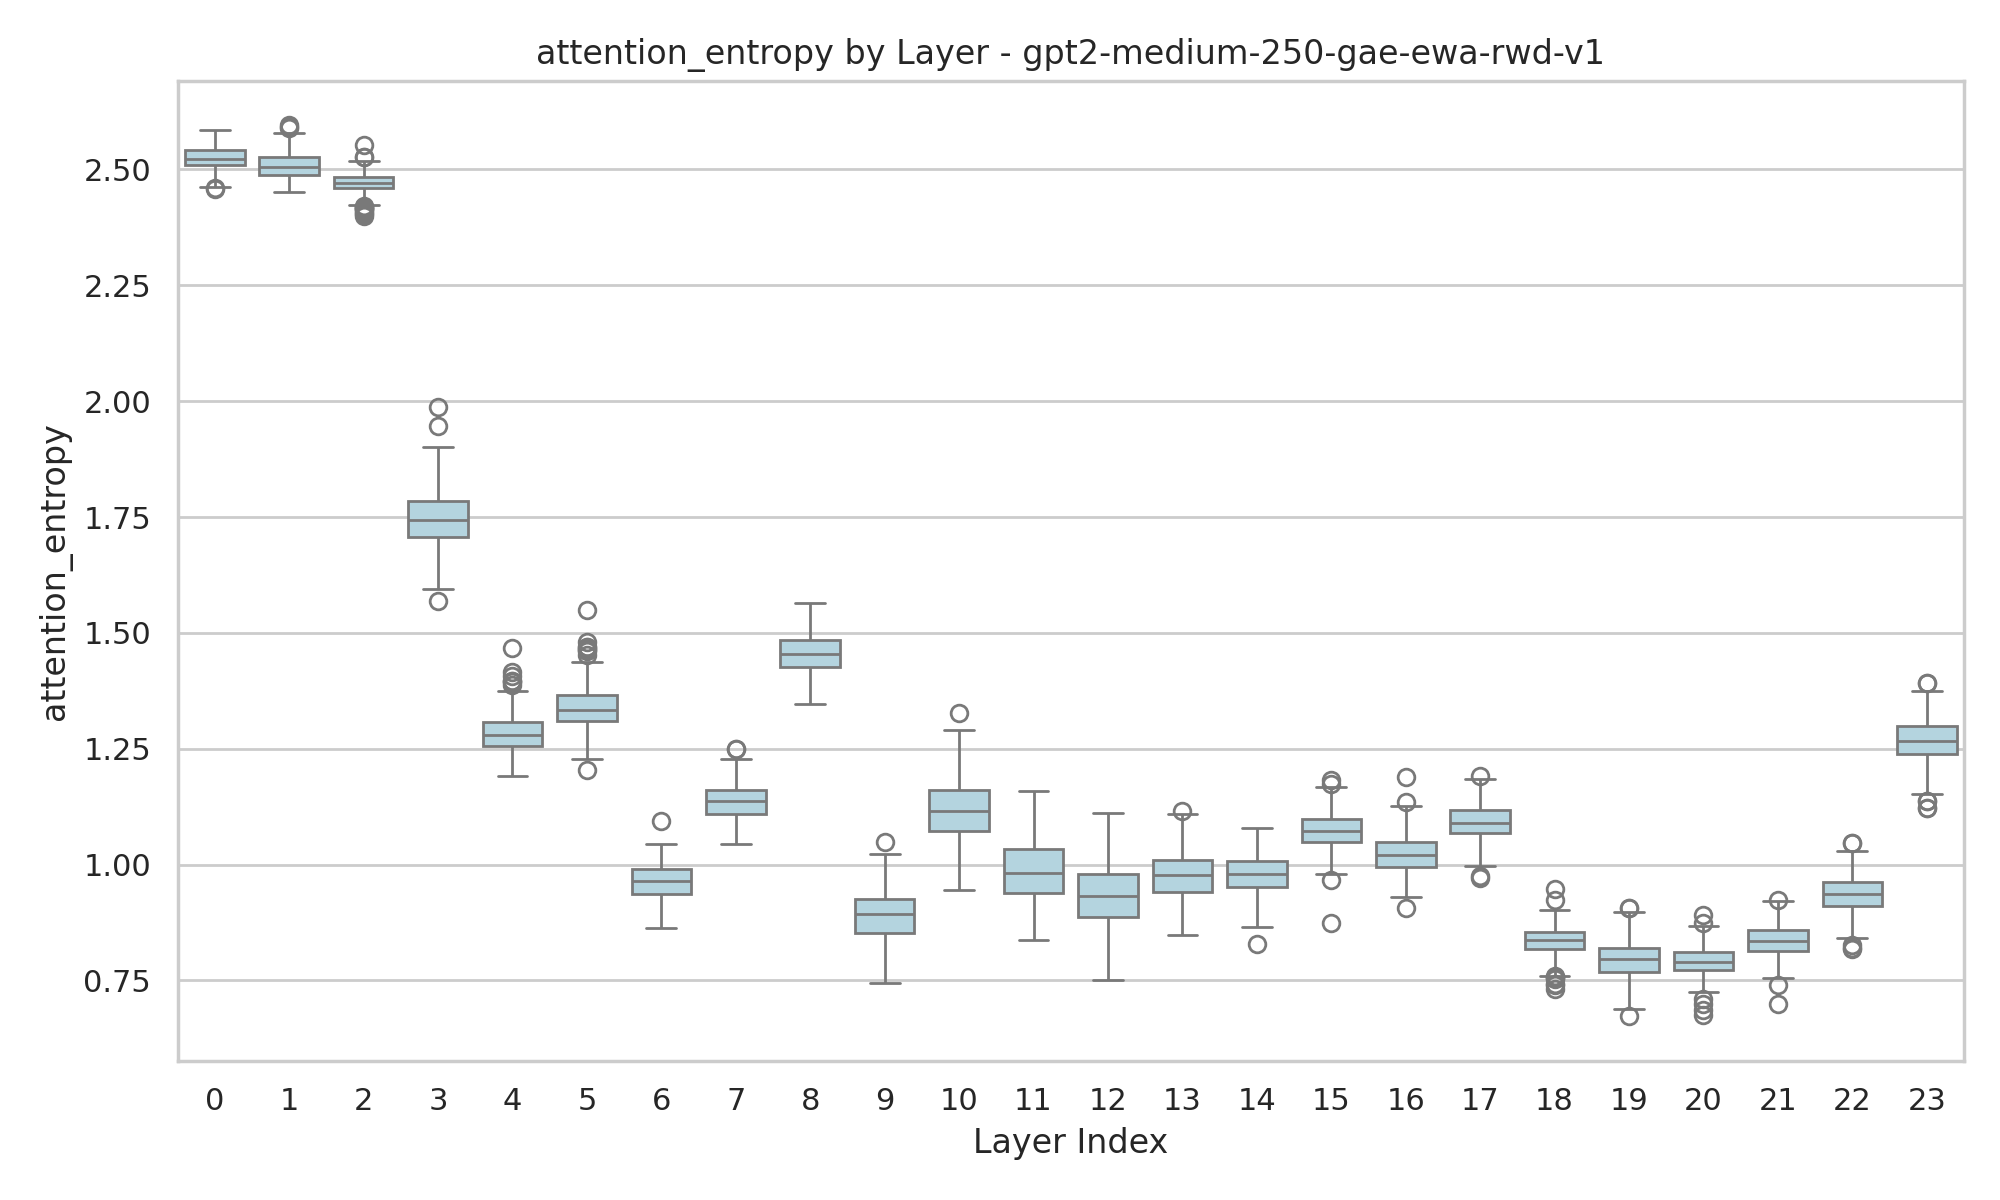
\includegraphics[width=1.0\linewidth]{gpt2-medium-250-gae-ewa-rwd-v1_layerstats_attention_entropy.png}
		\caption{\small
			\textbf{Attention Entropy Across Layers (GPT-2 Medium).}
			Each box shows the distribution of average attention entropy values for one layer, collected over multiple episodes. 
			Layers near the start (indices 0--2) exhibit higher entropy, possibly because they are attending to more general tokens, while deeper layers often have lower entropy, reflecting more specialized attention patterns.
		}
		\label{fig:gpt2medium-attn-entropy}
	\end{figure}
	
	\subsection{Distribution of Quant Types per Layer}
	\label{sec:medium-quant-dist}
	
	\begin{figure}[ht]
		\centering
		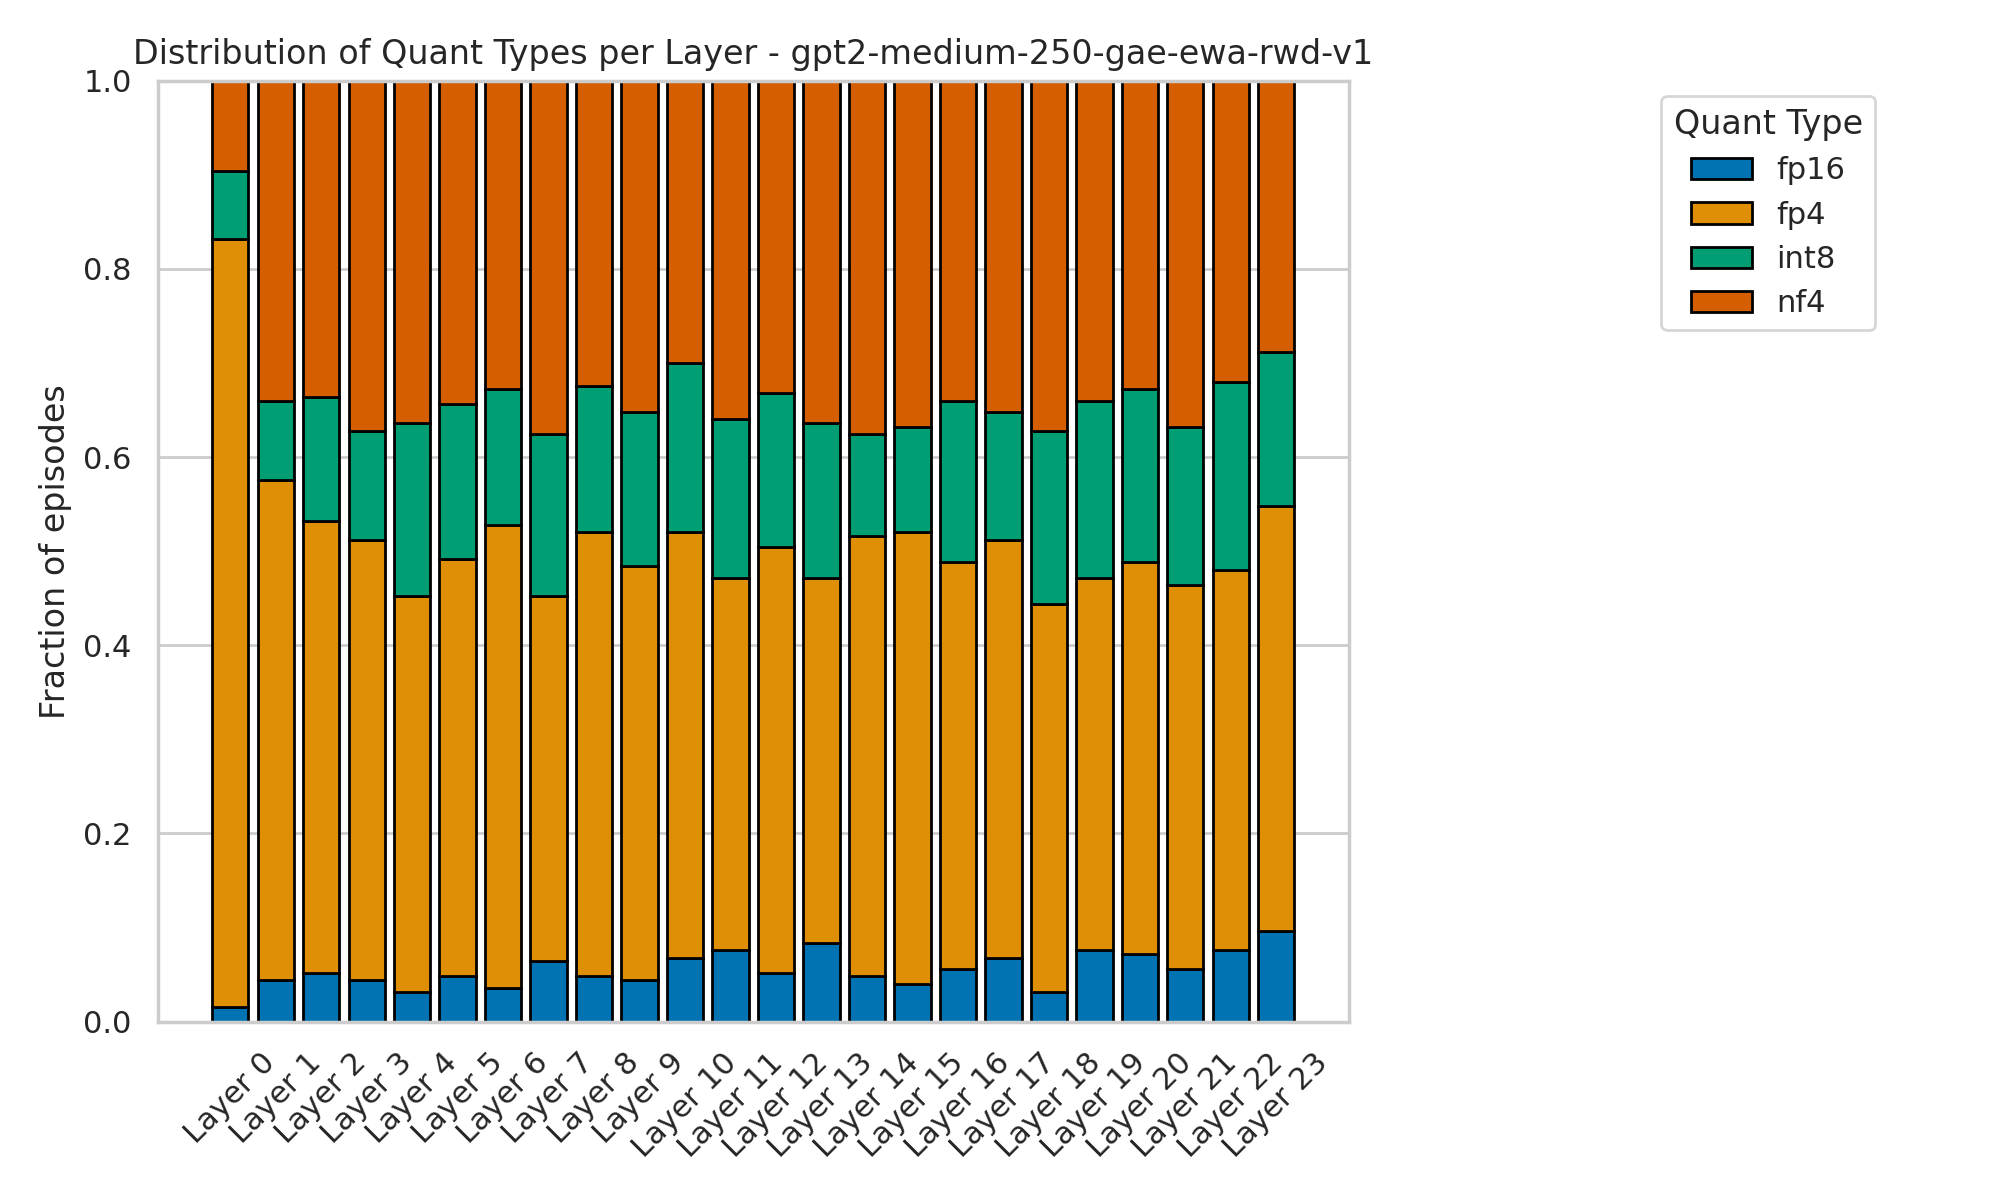
\includegraphics[width=0.85\linewidth]{gpt2-medium-250-gae-ewa-rwd-v1_quant_dist_bar.png}
		\caption{\small
			\textbf{Quantization Type Distribution.}
			For each layer index (horizontal axis), we show the fraction of training episodes (vertical) that chose a particular quant format (\texttt{fp16}, \texttt{fp4}, \texttt{int8}, \texttt{nf4}). 
			We see that middle layers (e.g.\ layers~5--15) are more heavily assigned 4-bit or 8-bit formats, whereas the first and last few layers sometimes remain at \texttt{fp16}.
		}
		\label{fig:gpt2medium-quant-dist}
	\end{figure}
	
	\subsection{Binned Quantization Heatmap}
	\label{sec:medium-heatmap}
	
	\begin{figure}[ht]
		\centering
		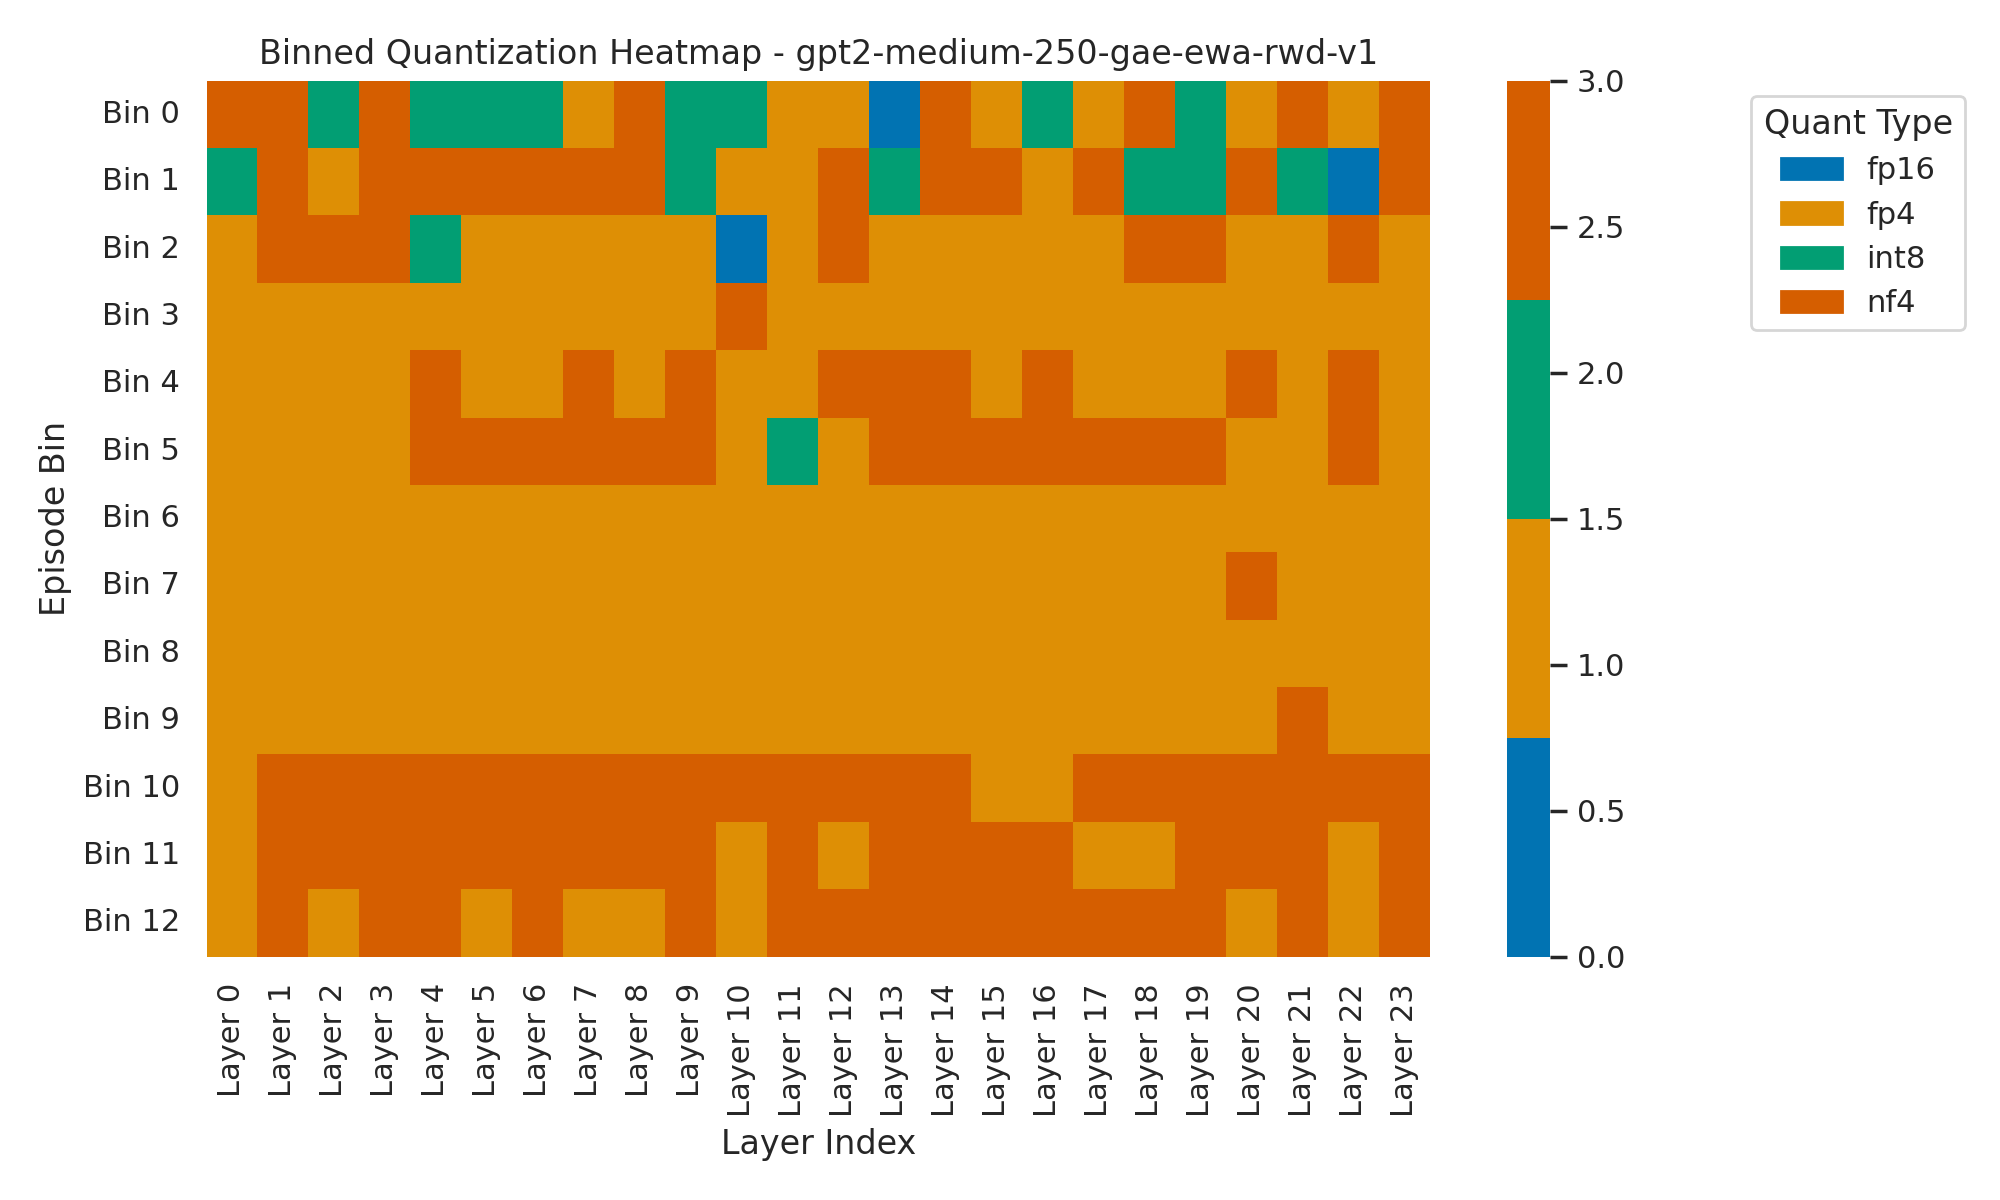
\includegraphics[width=1.0\columnwidth]{gpt2-medium-250-gae-ewa-rwd-v1_quant_heatmap_binned.png}
		\caption{\small
			\textbf{Quantization Heatmap by Episode Bin.}
			We group episodes in bins (vertical axis), and layers are shown horizontally. 
			The color indicates which quant type was chosen for that layer within each bin. 
			Early bins (top) show more exploration, while later bins (bottom) converge to a predominantly 4-bit strategy (orange), with occasional \texttt{int8} or \texttt{fp16} for sensitive layers.
		}
		\label{fig:gpt2medium-binned-heatmap}
	\end{figure}
	
	\subsection{Reward Components Over Episodes}
	\label{sec:medium-rewards}
	
	\begin{figure}[ht]
		
		\centering
		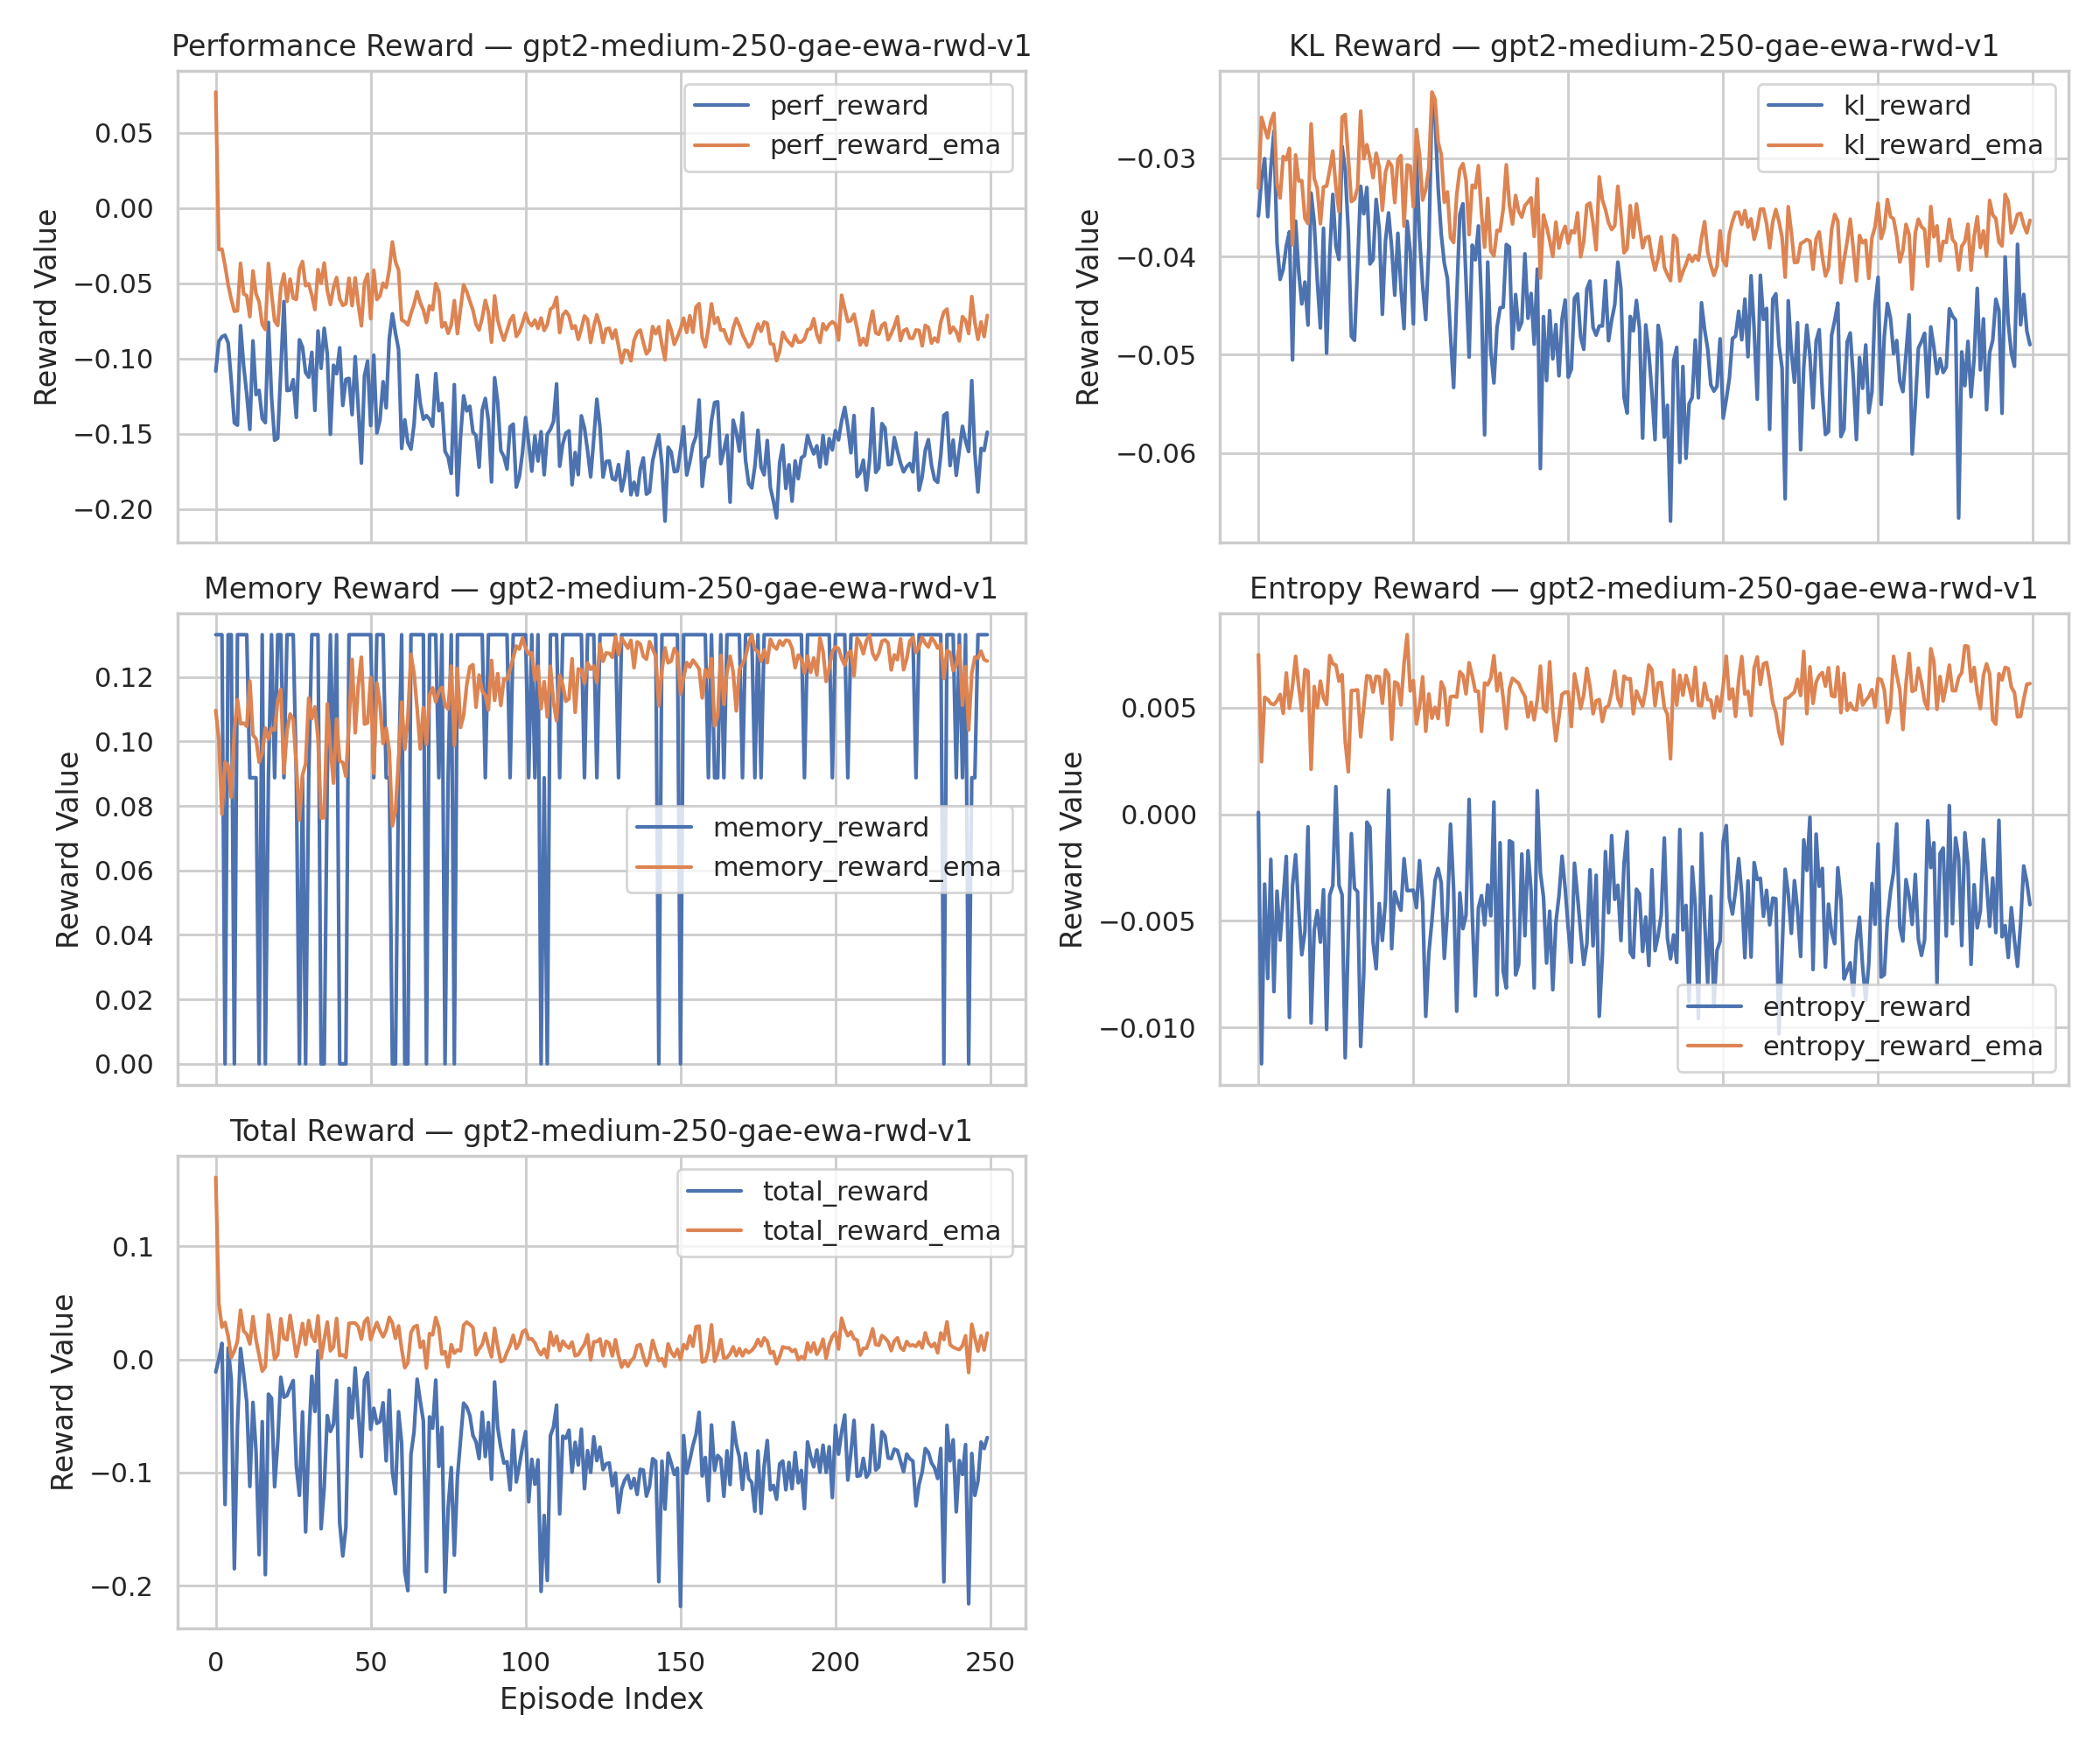
\includegraphics[width=1.0\columnwidth]{gpt2-medium-250-gae-ewa-rwd-v1_reward_subplots.png}
		\vspace{-1em}
		\caption{\small
			\textbf{Per-Episode Reward Components.}
			We log each reward component (performance, KL, memory, and entropy) as well as the total reward, in both raw (blue) and exponential moving average (orange) form. 
			Observe that memory rewards tend to remain positive (due to bit savings), while performance and KL can fluctuate or even be negative if a newly chosen quant format momentarily degrades perplexity or increases divergence. 
			Overall, the total reward stabilizes around a slightly positive mean, indicating a balanced trade-off across the four objectives.
		}
		\label{fig:gpt2medium-rewards}
	\end{figure}
	
	\vspace{1em}
	\noindent
	As shown in these figures, the RL policy for GPT-2 Medium (in this experiment) typically pushes \emph{more} layers toward low-bit formats (NF4 or FP4), but preserves higher precision in early and late layers where it observes larger sensitivity in perplexity or attention changes. 
	The reward breakdown confirms that while performance and KL terms sometimes turn negative after quantizing a “fragile” layer, the net reward remains moderately positive thanks to memory savings and stable attention patterns.
				
				
	
\end{document}
